\documentclass{beamer}
%\documentclass[presentation]{beamer}

\usecolortheme{Imperial}
 
\usepackage[utf8]{inputenc}
\usepackage[UKenglish]{babel}
\usepackage{booktabs}
\usepackage{caption}
\usepackage{subcaption}
\usepackage{graphicx}
\usepackage{amsmath}
\usepackage{amsfonts}
\usepackage{amssymb}
\usepackage{epstopdf}
\usepackage{tabularx}
    \newcolumntype{L}{>{\raggedright\arraybackslash}X}

% complying UK date format, i.e. 1 January 2001
\usepackage{datetime}
\let\dateUKenglish\relax
\newdateformat{dateUKenglish}{\THEDAY~\monthname[\THEMONTH] \THEYEAR}

% Imperial College Logo, not to be changed!
\institute{
\includegraphics[height=0.7cm]{Imperial_1_Pantone_solid.eps}}

% -----------------------------------------------------------------------------




%Information to be included in the title page:
\title{Learning Invariances in Dynamical System}

\subtitle{supervised by Dr Andrew Duncan and Dr Mark van der Wilk}

\author{Cheng-Cheng Lao}

\date{\today}



\begin{document}
 
\frame{\titlepage}

\begin{frame}
	\frametitle{Dynamical System}
\only<1>{
$$
m\frac{d^2x}{dt^2}+b\frac{dx}{dt}+kx=0,
$$}

\onslide<2->{
$$
\frac{d^{n} x}{d t^{n}}=F\left(t, x, \frac{d x}{d t}, \ldots, \frac{d^{n-1} x}{d t^{n-1}}\right),
$$
$$
\begin{cases}
  \dot{x}_1=f_1(x_1, \dots, x_n)\\ 
  \vdots\\
  \dot{x}_n=f_n(x_1, \dots, x_n)\\ 
\end{cases}
$$
}
\onslide<3->{
Planetary Evolution; Predator-Prey Dynamics, Protein mechanics, Quantum Mechanics

}
\end{frame}

\begin{frame}{Symmetry and Invariances}

	
\end{frame}


\begin{frame}
	\frametitle{Gaussian Process (GP)}
	\only<1>{\begin{definition}\begin{quote}GP is a collection of random variables, any finite number of which have a joint Gaussian distribution\end{quote}
	\end{definition}}
\only<2-4>{
$$
\begin{bmatrix}
  f\\f^*
\end{bmatrix}
\sim \mathcal{N}
\left(\mathbf{0}, \begin{bmatrix}K(X, X) & K(X, X^*) \\ K(X^*, X) & K(X^*, X^*) \end{bmatrix}\right),
$$
}
\only<3-4>{$$y=f+\epsilon;\ \epsilon\sim\mathcal{N}(0, \sigma^2_n)$$}
\onslide<4->{
$$
\begin{bmatrix}
  y\\f^*
\end{bmatrix}
\sim \mathcal{N}
\left(\mathbf{0}, \begin{bmatrix}K(X, X)+\sigma^2_n\mathbb{I} & K(X, X^*) \\ K(X^*, X) & K(X^*, X^*) \end{bmatrix}\right).
\label{equ:joint_gp_noise}
$$}
	\onslide<5->{
		A very important formula:
$$
  \text{if }
  \begin{bmatrix}
    x\\y
  \end{bmatrix} 
  \sim \mathcal{N}
  \left(
    \begin{bmatrix}
      \mathbf{\mu}_x\\
      \mathbf{\mu}_y
    \end{bmatrix},
    \begin{bmatrix}
      A & C \\
      C^T & B\\
    \end{bmatrix}
  \right), 
$$ 
		$$
  x|y\sim \mathcal{N}\left(\mathbf{\mu}_x+CB^{-1}(y-\mathbf{\mu}_y),A-CB^{-1}C^T\right)
  \label{equ:normal_condtion}
 $$
	}
	\onslide<6->{$$
\begin{gathered}
f^*|X, y, X^* \sim \mathcal{N} \left(\overline{f^*}, \mathrm{cov}(f^*)\right)\\ 
\overline{f^*} = K(X^*, X)[K(X,X)+\sigma^2_n\mathbb{I}]^{-1}y\\
\mathrm{cov}(f^*) = K(X^*, X^*) - K(X^*, X)[K(X, X)+\sigma^2_n\mathbb{I}]^{-1}K(X, X^*)
\end{gathered}
	$$}
	\onslide<7->{
$$
\log p(\mathbf{y} \mid X)=-\frac{1}{2} \mathbf{y}^{\top}\left(K+\sigma_{n}^{2} \mathbf{I}\right)^{-1} \mathbf{y}-\frac{1}{2} \log \left|K+\sigma_{n}^{2} \mathbf{I}\right|-\frac{n}{2} \log 2 \pi.
$$
	}
\end{frame}
\begin{frame}{Kernel}
	\only<1>{
		$$
  \begin{gathered}
    k_{RBF}(r) = \exp(-\frac{r^2}{2l^2}) \\
    k_{\text {Matérn}}(r)=\frac{2^{1-\nu}}{\Gamma(\nu)}\left(\frac{\sqrt{2 \nu} r}{\ell}\right)^{\nu} K_{\nu}\left(\frac{\sqrt{2 \nu} r}{\ell}\right) \\
    k_{periodic\ RBF}(r)=\exp \left(-\frac{2 \sin ^{2}\left(\frac{r}{2}\right)}{\ell^{2}}\right),
  \end{gathered}
		$$
	}
\only<2>{
\begin{figure}[H] 
  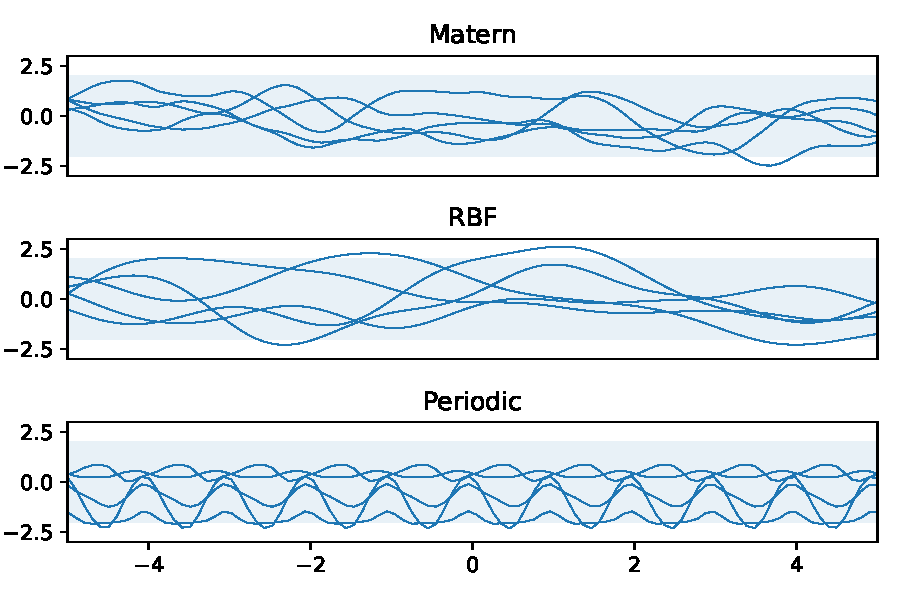
\includegraphics[width=0.7\linewidth]{../figures/prior.pdf}
  \centering
  \caption{Samples from different GP priors of RBF, Matérn and periodic kernel. }
  \label{fig:prior}
\end{figure}}
\end{frame}

\begin{frame}{GP regression in action}
	\onslide<1->{
		If we would like to fit a function $y=(x+x^2)\sin(x)$.
	\begin{figure}[H] 
	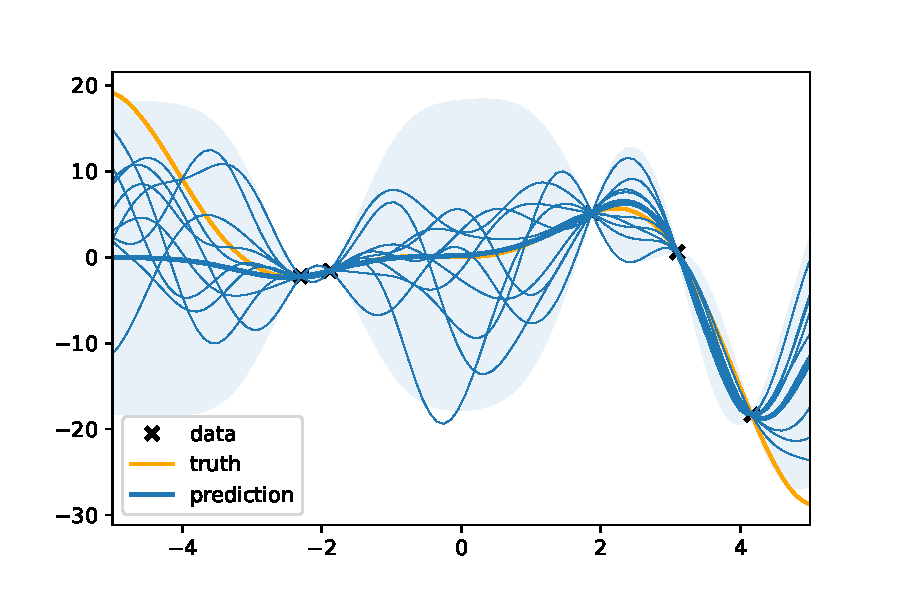
\includegraphics[width=0.7\linewidth]{../figures/posterior.pdf}
	\centering
	\caption{GP fit of the function $f=(x+x^2)\sin(x)$ with posterior samples, light shaded blue indicates 95\% credible interval.}
	\label{fig:posterior}
	\end{figure}

	}
	
\end{frame}
\begin{frame}{Related Work}
\begin{table}[H]
    \centering
\begin{tabularx}{\linewidth}{c|LLL} 
    \hline
 Methods & Respect the physics laws & Learn the physics laws & Generalise beyond physics   \\ 
    \hline
  ODE approach & X & O & O \\
  Symbolic approach & O & O & X \\
  Physics informed ML & O & X & X \\
  Energy conserving NN & O & X & X \\
  GP in dynamical system & X & O & O\\
  Our method & O & O & O\\
    \hline
\end{tabularx}
\caption{Comparing the capabilities of different existing approach to learning invariance in dynamical systems}
    \end{table}
\end{frame}

\begin{frame}{Invariance Kernel I}
	\onslide<1->{We have a general dynamical system with coordinates $\mathbf{p}, \mathbf{q}$, then we will call the dynamics $\frac{d\mathbf{p}}{dt}=a(\mathbf{p, q})$} and $\frac{d\mathbf{q}}{dt}=v(\mathbf{p, q})$.
	\onslide<2->{We will have $$\mathbf{f(\mathbf{q}, \mathbf{p})}=\begin{pmatrix}
    \mathbf{a(\mathbf{q}, \mathbf{p})}\\\mathbf{v(\mathbf{q}, \mathbf{p})}
\end{pmatrix}$$
}
	\onslide<3->{We will then put a GP prior on $\mathbf{f}$ so that $$\mathbf{f}\sim\mathcal{GP}(m, K)$$}
	
\end{frame}

\begin{frame}{Invariance Kernel II}
	\only<1-2>{$$X\equiv\begin{pmatrix}
    \mathbf{x}_1\\\vdots\\\mathbf{x}_n
\end{pmatrix}=\begin{pmatrix}
    q_{11}& q_{21} &\dots& q_{d1} & p_{11} & p_{21} & \dots & p_{d1} \\
    \vdots &\vdots &\ddots &\vdots &\vdots &\vdots &\ddots &\vdots \\
    q_{1n}& q_{2n} &\dots& q_{dn} & p_{1n} & p_{2n} & \dots & p_{dn} \\
\end{pmatrix}.$$
}
\only<2>{$$\mathbf{f}(X)=\begin{pmatrix}
    a_1(\mathbf{x}_1)\\
    \vdots\\
    a_1(\mathbf{x}_n)\\
    \vdots\\
    a_d(\mathbf{x}_n)\\
    v_1(\mathbf{x}_1)\\
    \vdots\\
    v_d(\mathbf{x}_n)\\
\end{pmatrix}$$}
\onslide<3->{
$$K=\mathrm{Cov}(\mathbf{f}(X), \mathbf{f}(X'))=
$$
$$
\begin{pmatrix}
    K_{a_1}(X,X') & \dots  & \dots          & \dots         & 0\\
    \vdots        & \ddots & \dots          & \ddots        & \vdots\\
    0             & \dots  & K_{a_d}(X,X')  & \dots         & 0 \\
    \vdots        & \ddots & \vdots         & K_{v_1}(X,X') & \vdots \\
    0             & \dots  & 0              & \dots         & K_{v_d}(X,X')\\
\end{pmatrix},
$$
where each $K_{f}$ is an RBF kernel}
\end{frame}
\begin{frame}{Invariance Kernel III}
	\onslide<1->{
\begin{equation*}
\mathcal{L}[E] \equiv \frac{dE}{dt}=\sum_{i=1}^d \frac{\partial E}{\partial p_i} \frac{\partial p_i}{\partial t}+ \sum_{i=1}^d\frac{\partial E}{\partial q_i}\frac{\partial q_i}{\partial t} 
\label{equ:LE}
\end{equation*}
$$=\sum_{i=1}^d \frac{\partial E}{\partial p_i} a_i(\mathbf{p,q}) + \sum_{i=1}^d\frac{\partial E}{\partial q_i} v_i(\mathbf{p,q})=L[\mathbf{f}]
$$
	}
	\onslide<2->{
$$
\begin{pmatrix}
\mathbf{f}(X)\\L[\mathbf{f}(X_L)]
\end{pmatrix}
\sim\mathcal{N}
\left(\begin{pmatrix}\mathbf{0}_{2nd}\\\mathbf{0}_{\ell}\end{pmatrix}, \begin{pmatrix}
    K & LK \\
    KL^T & LKL^T\\
\end{pmatrix}\right)
$$
\onslide<3->{
	$$
  \mathbf{f}(X)|L[\mathbf{f}(X_L)]=0 \sim \mathcal{N} \left(\mathbf{0}_{2nd}, \begin{pmatrix}
    K-LK(LKL^T)^{-1}KL^T
  \end{pmatrix}\right)$$
}
}
\end{frame}

\begin{frame}{Learning Invariance}
	\onslide<1->{
$$
\mathcal{L}[E] = \sum_{i=1}^d \frac{\partial E}{\partial p_i} a_i(\mathbf{p,q}) + \sum_{i=1}^d\frac{\partial E}{\partial q_i} v_i(\mathbf{p,q})
$$
	}
	\begin{itemize}
		\item \onslide<2->{One dimensional: $$L[\mathbf{f}]=f(p)a+g(q)v$$}
		\item \onslide<3->{Two dimensional: \begin{align*}
			L[\mathbf{f}]&=f_1(q_1, q_2, p_1, p_2)a_1+f_2(q_1, q_2, p_1, p_2)a_2\\&+g_1(q_1, q_2, p_1, p_2)v_1+g_2(q_1, q_2, p_1, p_2)v_2 
		\end{align*}}
	\end{itemize}
\end{frame}

\begin{frame}{Damped System- Approximate Invariance}
\onslide<1->{we have $L[\mathbf{f}(X_L)]=\epsilon$, where $\epsilon\sim\mathcal{N}(m_L, \sigma_L^2)$}
\onslide<2->{
$$
\begin{pmatrix}
\mathbf{f}(X)\\L[\mathbf{f}(X_L)]
\end{pmatrix}
\sim\mathcal{N}
\left(\begin{pmatrix}\mathbf{0}_{2nd}\\\mathbf{m}_{\ell}\end{pmatrix}, \begin{pmatrix}
    K & LK \\
    KL^T & LKL^T+\sigma_L^2\mathbb{I}\\
\end{pmatrix}\right),
$$
}
\end{frame}

\begin{frame}{Damped System- Latent Dynamics}
	\onslide<1->{
$$
\mathcal{L}[E] + z = \frac{dE}{dt} + z =\sum_{i=1}^d \frac{\partial E}{\partial p_i} \frac{\partial p_i}{\partial t}+ \sum_{i=1}^d\frac{\partial E}{\partial q_i}\frac{\partial q_i}{\partial t} + z = 
$$
$$
\sum_{i=1}^d \frac{\partial E}{\partial p_i} a_i + \sum_{i=1}^d\frac{\partial E}{\partial q_i} v_i + z=L_\gamma[\mathbf{f}_\gamma]=0
$$	
}
\onslide<2->{
	$$
\begin{pmatrix}
\begin{pmatrix}\mathbf{f}(X)\\ z(X)\end{pmatrix}\\L_\gamma[\mathbf{f}(X_L), z(X_L)]
\end{pmatrix}
\sim\mathcal{N}
\left(\begin{pmatrix}\mathbf{0}_{3nd}\\\mathbf{0}_{\ell}\end{pmatrix}, \begin{pmatrix}
    K & L_\gamma K \\
    KL_\gamma^T & L_\gamma KL_\gamma^T\\
\end{pmatrix}\right),
	$$
}
	
\end{frame}
\begin{frame}{Experiments}
	\begin{enumerate}
		\item Data Generation
		\item Evaluation Methods
		\item Implementation Techicalities
	\end{enumerate}
\end{frame}


\begin{frame}{Simple Harmonic Motion (SHM)}
	\onslide<1->{
		$$\frac{d^2x}{dt^2}=-\frac{kx}{m}$$
		$$x=A\sin(\omega_0t+\phi)$$
	}
	\only<2>{
\begin{figure}[H]
        \centering
        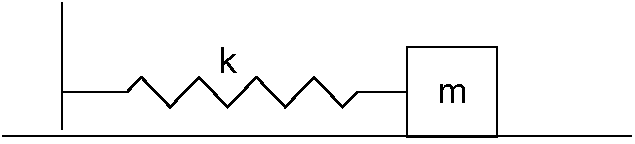
\includegraphics[width=0.8\linewidth]{../figures/shm.pdf}
\end{figure}
	}
	\onslide<3->{
\begin{figure}[H] 
  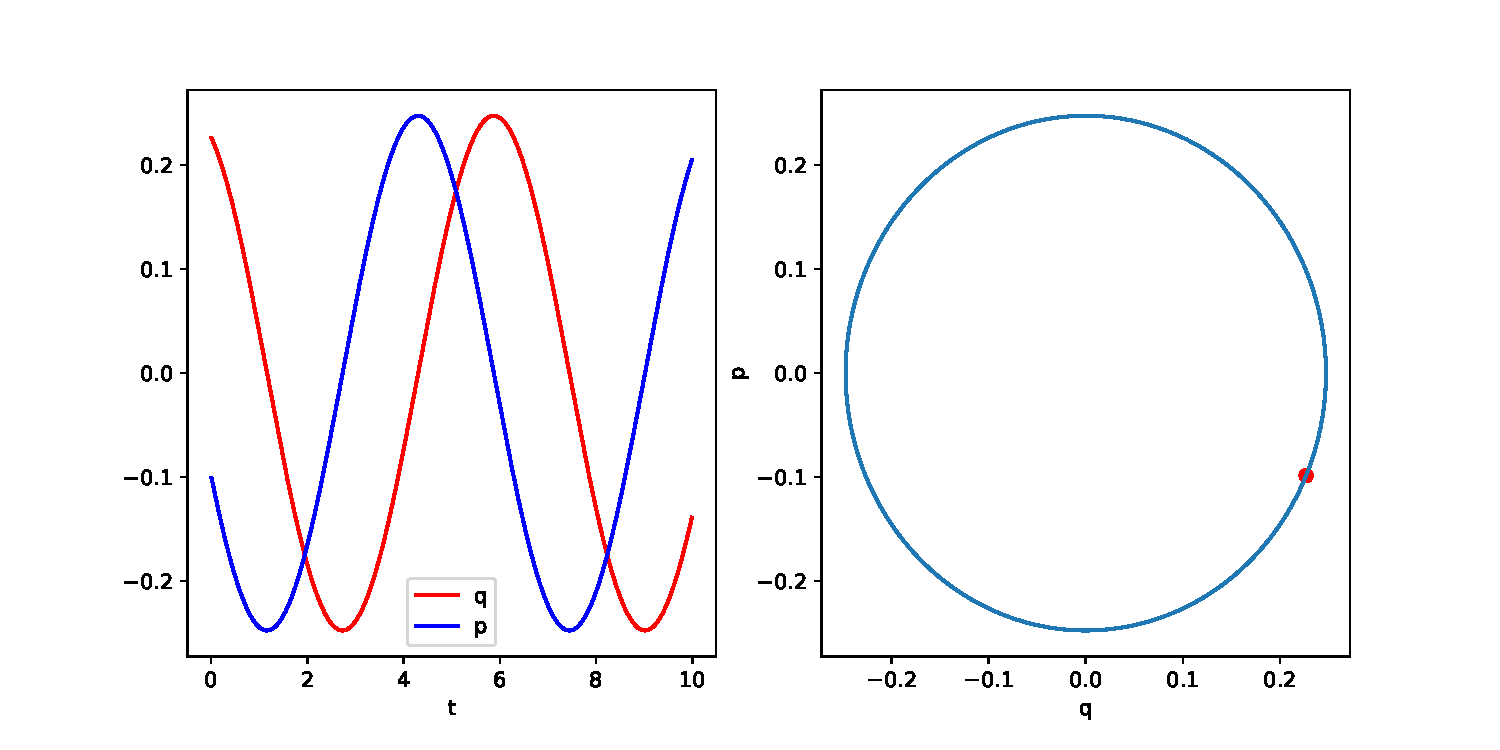
\includegraphics[width=0.7\linewidth]{../codes/figures/shm_trajectory_1D.pdf}
  \centering
\end{figure}
	}
\end{frame}

\begin{frame}{SHM Invariance Kernel- I}
	\onslide<1->{
$$
\text{We had } \mathcal{L}[E] \equiv \frac{dE}{dt}=\sum_{i=1}^d \frac{\partial E}{\partial p_i} a_i(\mathbf{p,q}) + \sum_{i=1}^d\frac{\partial E}{\partial q_i} v_i(\mathbf{p,q})=L[\mathbf{f}]
$$
	}
	\onslide<2->{$$E=\frac{kq^2}{2}+\frac{mp^2}{2}$$}
	\onslide<3->{So we have $$L[\mathbf{f}]=mpa+kvp=0$$}
	\onslide<4->{
$$
L([\mathbf{f}(X_L)]) = \begin{pmatrix}
   mp_{L,1}a(q_{L,1},p_{L,1}) + kq_{L,1}v(q_{L,1},p_{L,1})\\ 
   \vdots \\
   mp_{L,\ell}a(q_{L,\ell},p_{L,\ell}) + kq_{L,\ell}v(q_{L,\ell},p_{L,\ell})\\ 
\end{pmatrix},
$$
	}
\end{frame}

\begin{frame}{SHM Invariance Kernel- II}
	\only<1>{$$
\begin{pmatrix}
    \mathbf{f}(X)\\
    L([\mathbf{f}(X_L)])\\
\end{pmatrix}
\sim\mathcal{N}
\left(\begin{pmatrix}
    0_{2n}\\0_{\ell}
\end{pmatrix},\begin{pmatrix}
   A & B \\
   C & D\\ 
\end{pmatrix}\right)
	$$
$$
\mathbf{f}(X)|L[\mathbf{f}(X_L)]=0\sim\mathcal{N}(0_{2n},A-BD^{-1}C),
$$
	}
	\onslide<2->{$$
\begin{gathered}
A=K(X,X), B=\begin{pmatrix}
    K_{a}(X, X_L) \\ K_{v}(X, X_L) \\
\end{pmatrix}\odot \begin{pmatrix}
    mP_L \\ kQ_L
\end{pmatrix}, C=B^T,\\ D=K_{a}(X_L, X_L)\odot m^2(p_L\otimes p_L) + K_{v}(X_L, X_L)\odot k^2(q_L\otimes q_L),
\end{gathered}
	$$
$$
P_L=\begin{pmatrix}
  p_{L,1}  & \dots & p_{L,\ell}  \\
  \vdots & \text{repeats n rows} &  \vdots\\
  p_{L,1}  & \dots & p_{L,\ell}  \\
\end{pmatrix},
$$
$$
p_L\otimes p_L=\begin{pmatrix}
  p_{L,1}^2 & p_{L,1}p_{L,2} & \dots & p_{L,1}p_{L,\ell} \\
  \vdots & \vdots & \vdots & \vdots \\
  p_{L,\ell}p_{L,1} & p_{L,\ell}p_{L,2} & \dots & p_{L,\ell}^2 \\
\end{pmatrix},
$$ 
	}
\end{frame}

\begin{frame}{SHM Invariance Kernel- III}
	\only<1>{
\begin{align*}
B_{ij} &= \mathrm{Cov}(\mathbf{f}(X), L[\mathbf{f}(X_L)])_{ij} \\
       &= \mathrm{Cov}(\mathbf{f}(X)_i, L[\mathbf{f}(X_L)]_j) \\ 
       &= \begin{cases}
        \mathrm{Cov}(a(q_i, p_i), mp_{L,j}a(q_{L,j},p_{L,j}) + kq_{L,j}v(q_{L,j},p_{L,j})) & i\le n \\ 
        \mathrm{Cov}(v(q_i, p_i), mp_{L,j}a(q_{L,j},p_{L,j}) + kq_{L,j}v(q_{L,j},p_{L,j})) & i>n \\ 
       \end{cases} \\
       &= \begin{cases}
        K_{RBF,a}(\mathbf{x}_i, \mathbf{x}_{L,j}) mp_{L,j} & i\le n \\ 
        K_{RBF,v}(\mathbf{x}_i, \mathbf{x}_{L,j}) kq_{L,j} & i>n \\ 
       \end{cases}, \\
\end{align*}
	}
	\only<2>{
\begin{align*}
D_{ij} &= \mathrm{Cov}(L[\mathbf{f}(X_L)], L[\mathbf{f}(X_L)])_{ij} \\
       &= \mathrm{Cov}(mp_{L,i}a(q_{L,i},p_{L,i}) + kq_{L,i}v(q_{L,i},p_{L,i}), mp_{L,i}a(q_{L,i},p_{L,i}) + kq_{L,i}v(q_{L,i},p_{L,i})) \\
       &= m^2p_{L,i}p_{L,j}K_{RBF,a}(\mathbf{x}_{L,i},\mathbf{x}_{L,j}) + k^2q_{L,i}q_{L,j}K_{RBF,v}(\mathbf{x}_{L,i},\mathbf{x}_{L,j})
\end{align*}
	}
\end{frame}

\begin{frame}{Learning Invariance}
	\only<1>{
	$$	
 \mathcal{L}[E] \equiv \frac{dE}{dt}=\sum_{i=1}^d \frac{\partial E}{\partial p_i} a_i(\mathbf{p,q}) + \sum_{i=1}^d\frac{\partial E}{\partial q_i} v_i(\mathbf{p,q})=L[\mathbf{f}]
$$
	}
	\onslide<1->{
	$$L[\mathbf{f}]=f(p)a+g(q)v$$
	}
	\onslide<2->{$$
\begin{gathered}
A=K(X,X), B=\begin{pmatrix}
    K_{a}(X, X_L) \\ K_{v}(X, X_L) \\
\end{pmatrix}\odot \begin{pmatrix}
    f(P_L) \\ g(Q_L)
\end{pmatrix}, C=B^T,\\ D=K_{a}(X_L, X_L)\odot (f(p_L)\otimes f(p_L)) + K_{v}(X_L, X_L)\odot (g(q_L)\otimes g(q_L)),
\end{gathered}
 $$
	}
	\onslide<3->{
$$
f(P_L)=\begin{pmatrix}
  f(p_{L,1})  & \dots & f(p_{L,\ell})  \\
  \vdots & \text{repeats n rows} &  \vdots\\
  f(p_{L,1})  & \dots & f(p_{L,\ell})  \\
\end{pmatrix},
$$
$$
f(p_L)\otimes f(p_L)=\begin{pmatrix}
  f(p_{L,1})^2 & f(p_{L,1})f(p_{L,2}) & \dots & f(p_{L,1})f(p_{L,\ell}) \\
  \vdots & \vdots & \vdots & \vdots \\
  f(p_{L,\ell})f(p_{L,1}) & f(p_{L,\ell})f(p_{L,2}) & \dots & f(p_{L,\ell})^2 \\
\end{pmatrix},
$$
	}
	
\end{frame}

\begin{frame}{Results for SHM}
\only<1>{
\begin{table}[H]
  \centering
\begin{tabularx}{\linewidth}{l l L L} 
\hline
Method           & RBF & Known Invariance&  Learnt Invariance\\
  \hline
Log Marginal Likelihood & 67.67 & 82.00 & 79.24 \\
MSE & 0.0950 & 0.0017 & 0.0027 \\
                    \hline
  \end{tabularx}
  \caption{SHM performance.}
\end{table}}
\only<2>{
\begin{figure}[H]
        \centering
        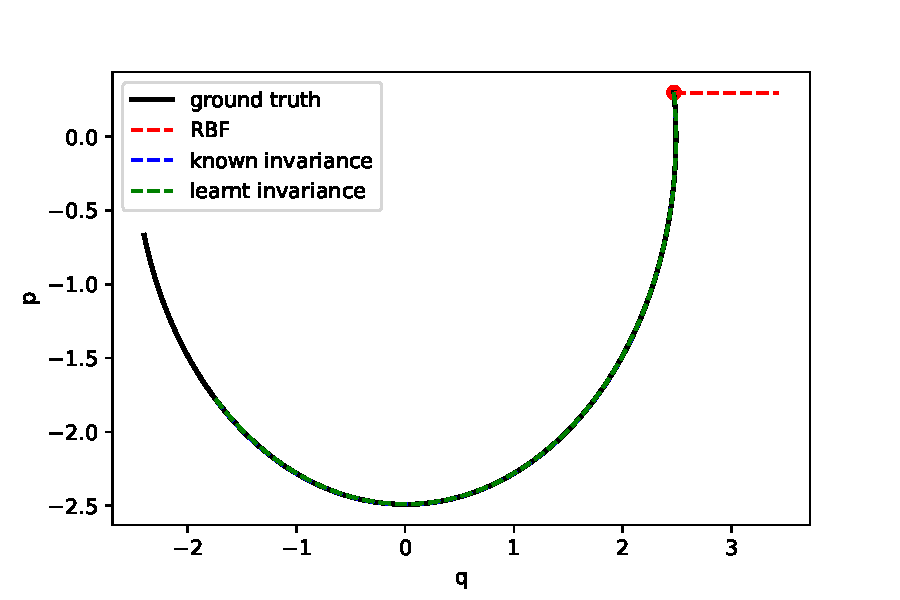
\includegraphics[width=0.8\linewidth]{../codes/figures/shm_predicted.pdf}
        \caption{One SHM predicted trajectory.}\end{figure}
}
\only<3>{

\begin{figure}[H] 
  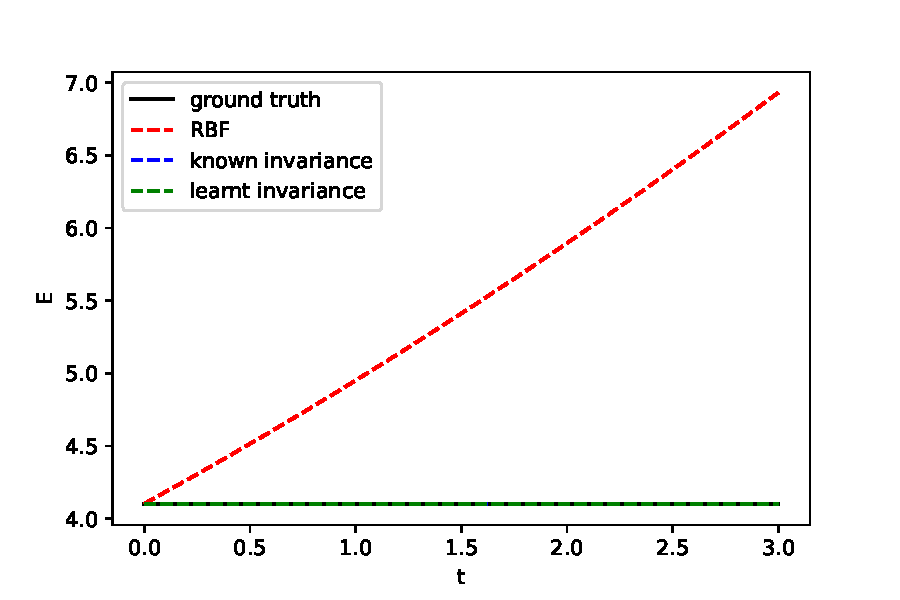
\includegraphics[width=0.8\linewidth]{../codes/figures/shm_energy.pdf}
  \centering
  \caption{The energy along the trajectory.}\end{figure}
}
\only<4>{
\begin{figure}[H]
        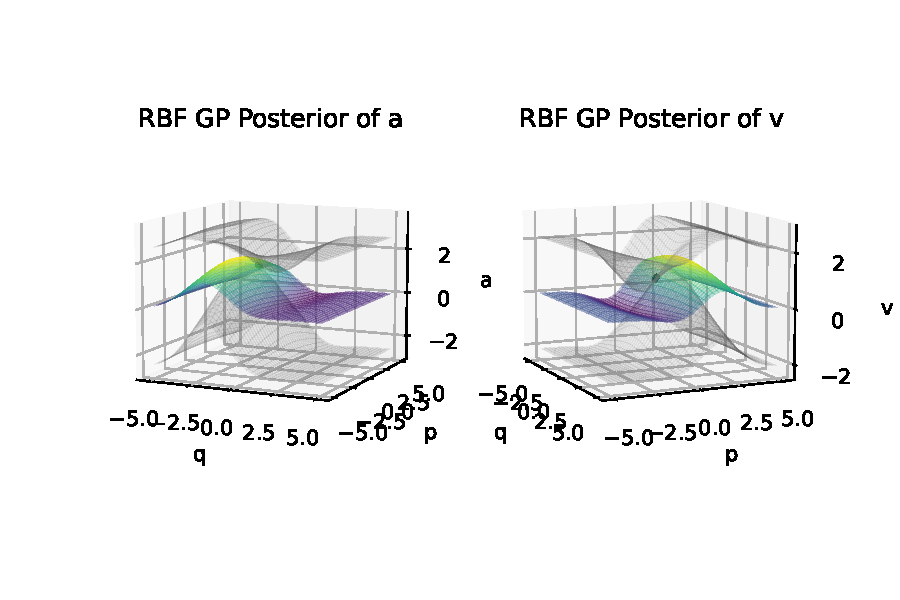
\includegraphics[width=\linewidth]{../codes/figures/posterior_shm_rbf.pdf}
     \centering
        \caption{SHM RBF posterior}
\end{figure}

}
\only<5>{
\begin{figure}[H]
         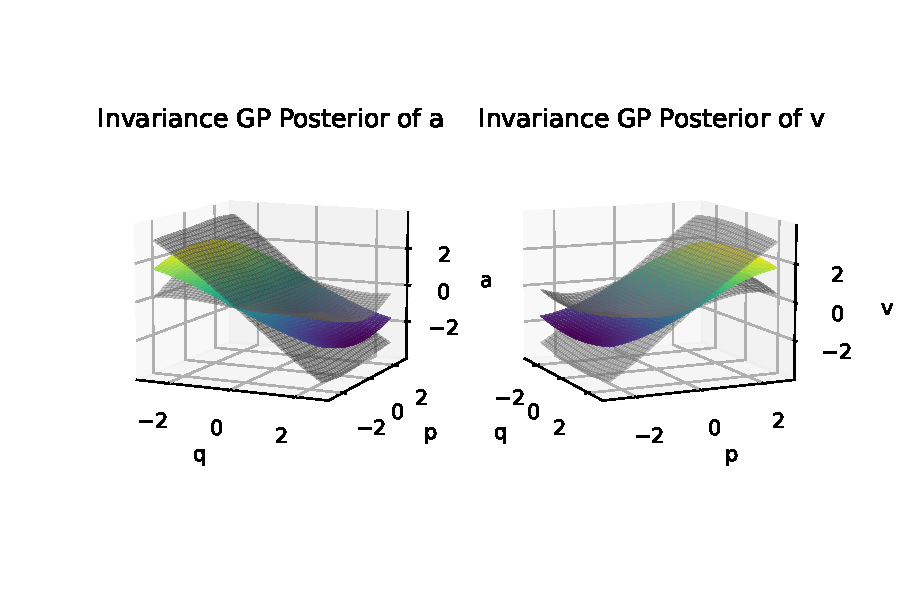
\includegraphics[width=\linewidth]{../codes/figures/posterior_shm_invariance.pdf}
	\centering
         \caption{SHM invariance posterior}
\end{figure}
}
\only<6>{
\begin{figure}[H] 
  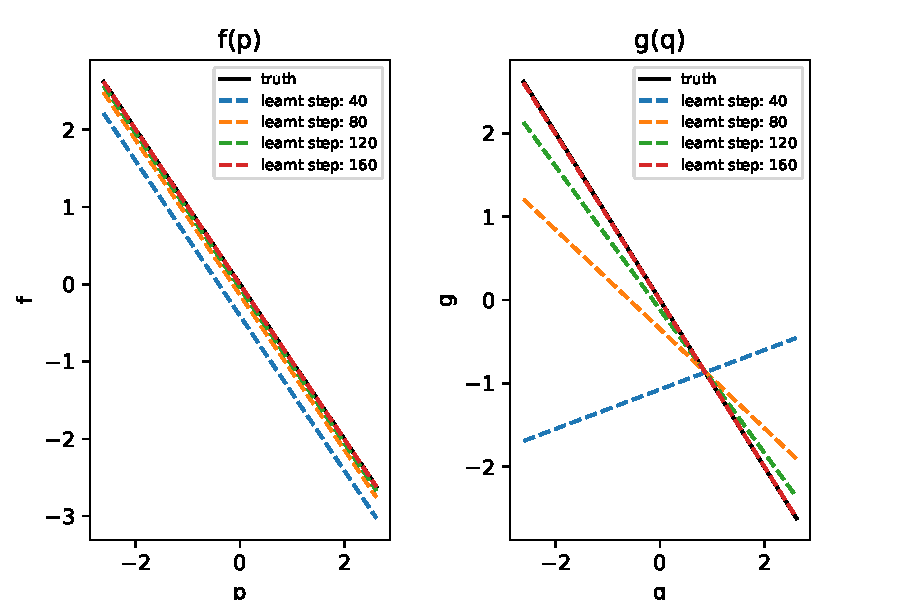
\includegraphics[width=0.8\linewidth]{../codes/figures/shm_learnt_over_time.pdf}
  \centering
  \caption{Learnt invariance for SHM.} \end{figure}


}


\end{frame}

\begin{frame}{Pendulum}
	\onslide<1->{
$$
\frac{d^2q}{dt^2}=-\frac{g}{\ell}\sin q, 
$$}
\only<2>{
\begin{figure}[H]
        \centering
        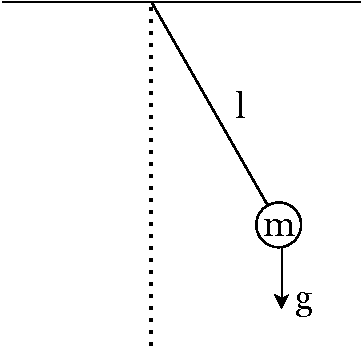
\includegraphics[width=0.3\linewidth]{../figures/pendulum.pdf}
        \caption{A pendulum is a simple system that is nonlinear.}
\end{figure}
}
\onslide<3->{

\begin{figure}[H] 
  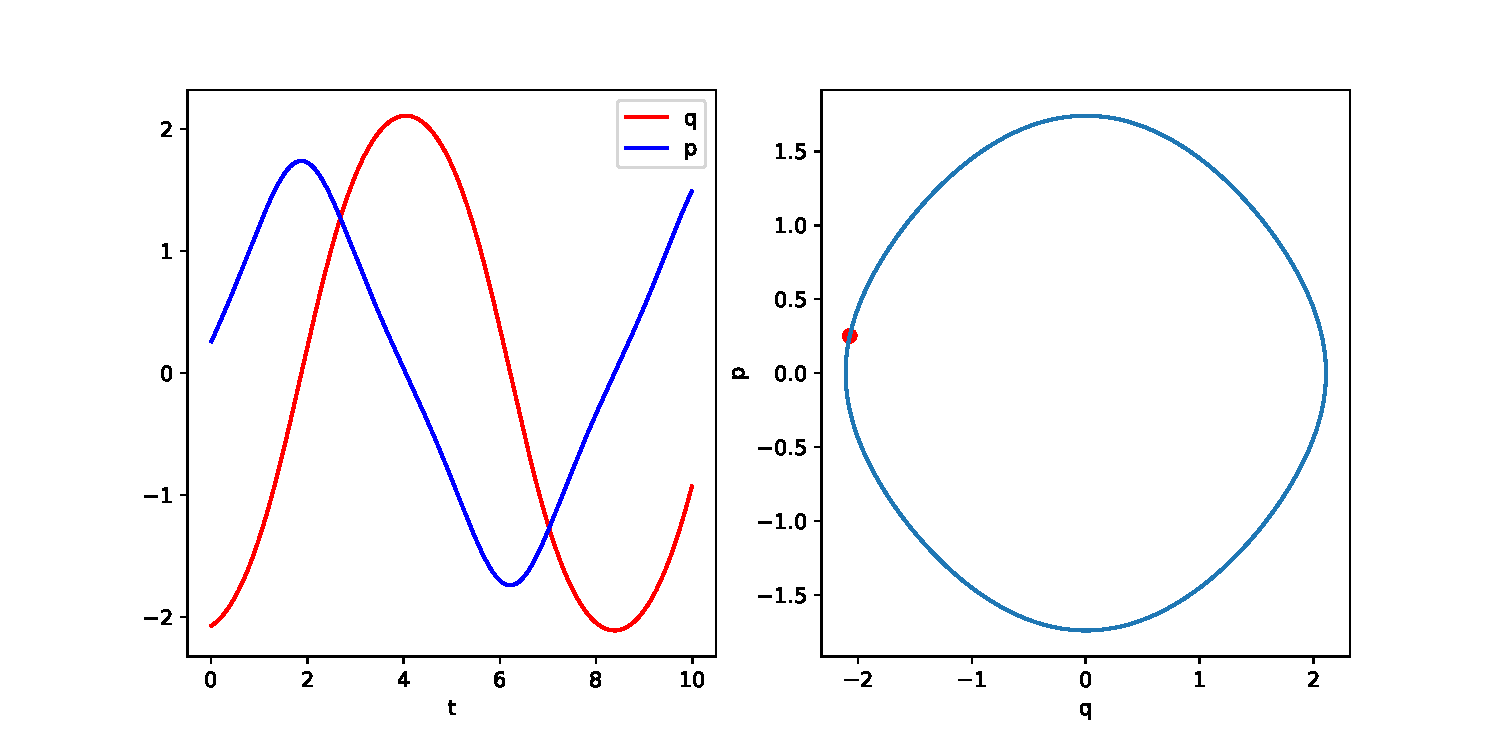
\includegraphics[width=0.7\linewidth]{../codes/figures/pendulum_trajectory_1D.pdf}
  \centering
  \caption{Example trajectory of pendulum.} \end{figure}
}

\end{frame}

\begin{frame}{Pendulum Invariance}
	\only<1-3>{
	$$	
 \mathcal{L}[E] \equiv \frac{dE}{dt}=\sum_{i=1}^d \frac{\partial E}{\partial p_i} a_i(\mathbf{p,q}) + \sum_{i=1}^d\frac{\partial E}{\partial q_i} v_i(\mathbf{p,q})=L[\mathbf{f}]
$$
	}
	\only<2-3>{
		$$E=\frac{m\ell^2p^2}{2}+mg\ell(1-\cos q)$$
	}
	\onslide<3->{
$$L[\mathbf{f}]=\ell pa+g(\sin q)v=0$$
	}
	\onslide<4->{$$
\begin{gathered}
B=\begin{pmatrix}
    K_{a}(X, X_L) \\ K_{v}(X, X_L) \\
\end{pmatrix}\odot \begin{pmatrix}
    \ell P_L \\ g\sin(Q_L)
\end{pmatrix},\\ D=K_{a}(X_L, X_L)\odot \ell^2(p_L\otimes p_L) + K_{v}(X_L, X_L)\odot g^2(\sin(q_L)\otimes \sin(q_L)),
\end{gathered}
$$
	}
	\onslide<5->{
$$
\sin(Q_L) = g\begin{pmatrix}
  \sin(q_{L,1})  & \dots & \sin(q_{L,\ell})  \\
  \vdots & \text{reqeats n rows} &  \vdots\\
  \sin(q_{L,1})  & \dots & \sin(q_{L,\ell})  \\
\end{pmatrix},
$$
$$
\sin(q_L)\otimes \sin(q_L)=\begin{pmatrix}
  \sin(q_{L,1})^2  \dots & \sin(q_{L,1})\sin(q_{L,\ell}) \\
  \vdots & \vdots & \vdots \\
  \sin(q_{L,\ell})\sin(q_{L,1}) &  \dots & \sin(q_{L,\ell})^2 \\
\end{pmatrix},
$$
	}
\end{frame}

\begin{frame}{Results for Pendulum}
\only<1>{
\begin{table}[H]
  \centering
\begin{tabularx}{\linewidth}{l l L L} 
\hline
Method           & RBF & Known Invariance&  Learnt Invariance\\
  \hline
Log Marginal Likelihood & 299.12 & 331.66 & 325.76 \\
MSE & 0.0021 & 0.0009 & 0.0006 \\
                    \hline
  \end{tabularx}
  \caption{Pendulum performance.}
\end{table}}
\only<2>{
\begin{figure}[H]
        \centering
        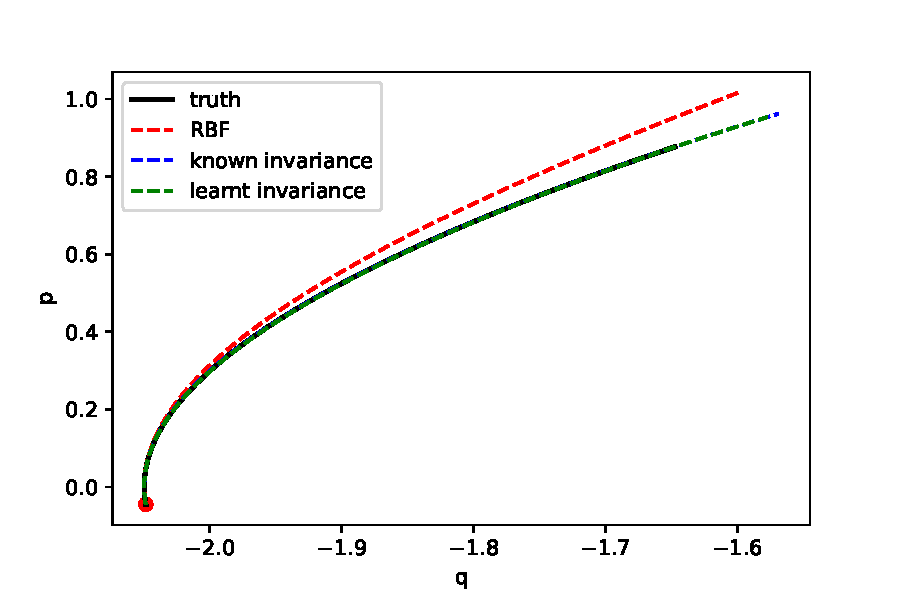
\includegraphics[width=0.8\linewidth]{../codes/figures/pendulum_predicted.pdf}
        \caption{Pendulum predicted trajectory.}\end{figure}
}
\only<3>{

\begin{figure}[H] 
  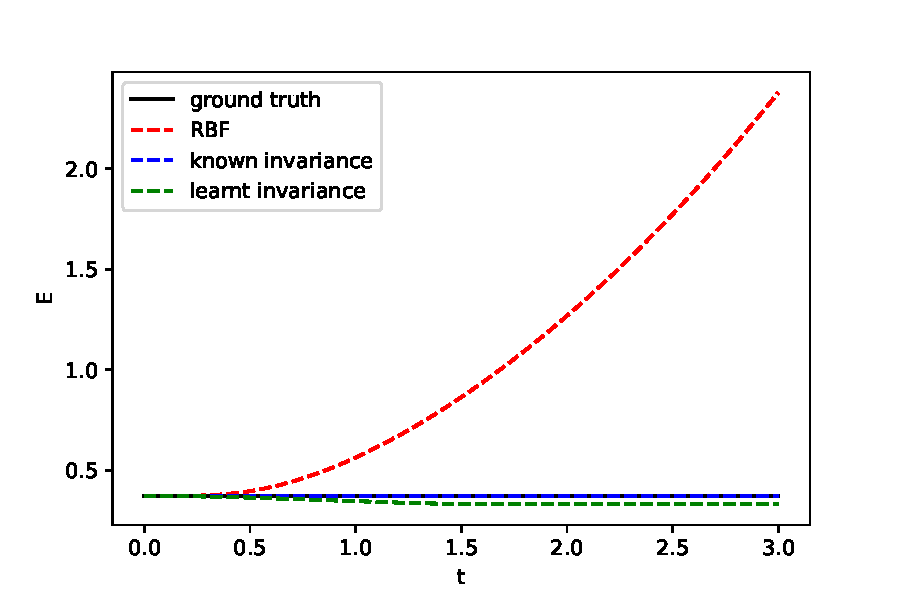
\includegraphics[width=0.8\linewidth]{../codes/figures/pendulum_energy.pdf}
  \centering
  \caption{The energy along the trajectory.}\end{figure}
}
\only<4>{
\begin{figure}[H]
         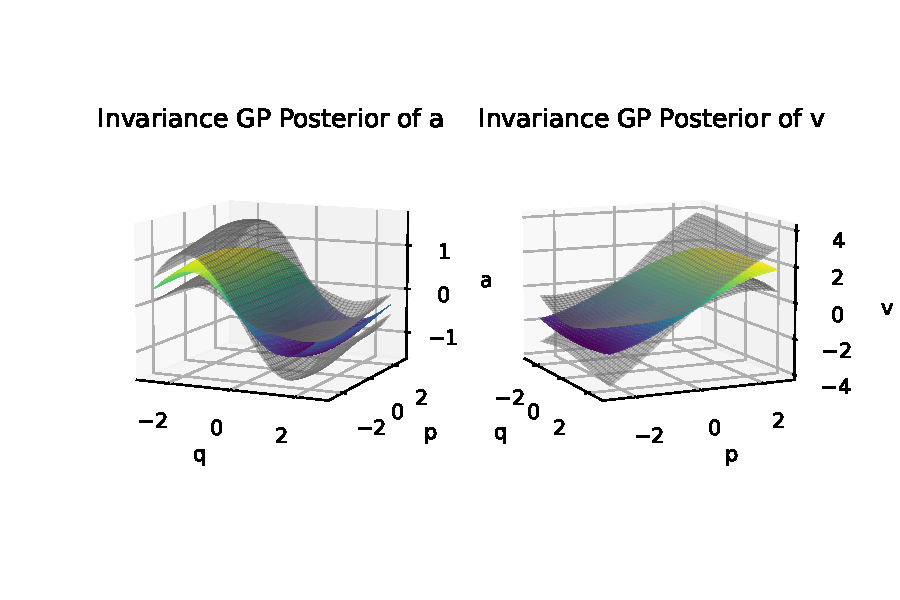
\includegraphics[width=\linewidth]{../codes/figures/posterior_pendulum_invariance.pdf}
	\centering
         \caption{Pendulum invariance posterior}
\end{figure}
}
\only<5>{
\begin{figure}[H] 
  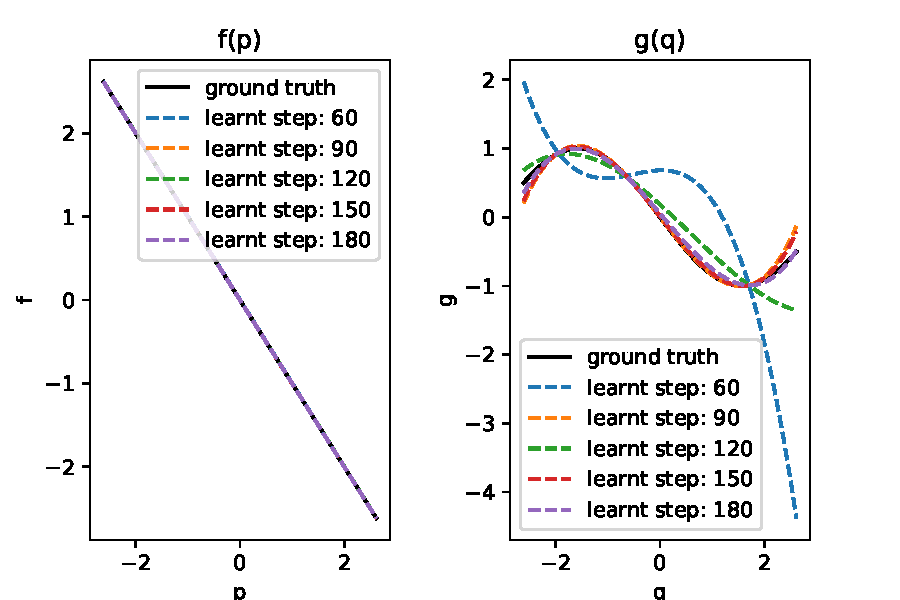
\includegraphics[width=0.8\linewidth]{../codes/figures/pendulum_learnt_over_time.pdf}
  \centering
  \caption{Learnt invariance for pendulum.} \end{figure}


}


	
\end{frame}


\begin{frame}{Damped Systems}
\onslide<1->{
$$
\frac{d^2q}{dt^2}+2\gamma\frac{dq}{dt}+\omega_0^2q=0;\ \frac{d^2q}{dt^2}+2\gamma\frac{dq}{dt}+\omega_0^2\sin q=0 ,
$$}
	
\end{frame}

	




\begin{frame}
	\frametitle{Two Figures aside}
	\begin{columns}[b]
		\column{0.0125\textwidth}
		\column{0.4875\textwidth}
			\centering
			\begin{figure}
				\includegraphics[draft,width=\textwidth]{fooA.pdf} \
				% remove the 'draft' keyword, when replacing with final figure!
				\caption{Caption of Figure A}
			\end{figure}
		\column{0.4875\textwidth}
			\centering
			\begin{figure}
				\includegraphics[draft,width=\textwidth]{fooB.pdf} \
				% remove the 'draft' keyword, when replacing with final figure!
				\caption{Caption of Figure B}
			\end{figure}
		\column{0.0125\textwidth}
	\end{columns}
\end{frame}


\begin{frame}
	\frametitle{Text and Figure aside}
	\begin{columns}[]
		\column{0.0125\textwidth}
		\column{0.4875\textwidth}
			\centering
			\begin{figure}
				\includegraphics[draft,width=\textwidth]{fooC.pdf} \
				% remove the 'draft' keyword, when replacing with final figure!
				\caption{Caption of Figure C}
			\end{figure}
		\column{0.4875\textwidth}
			Some text and a bullet point list
			\begin{itemize}
				\item ItemA
				\item ItemB
				\item ItemC
				\item ItemD
			\end{itemize}			
		\column{0.0125\textwidth}
	\end{columns}
\end{frame}


\begin{frame}
	\frametitle{One Figure}
	\bigskip
	\begin{figure}
		\includegraphics[draft,width=0.8\textwidth, height=0.5\textwidth]{fooD.pdf}
		% remove the 'draft' keyword, when replacing with final figure!
		\caption{Caption of Figure D}
	\end{figure}
\end{frame}

 
\end{document}
